\graphicspath{{pict}}
\DeclareGraphicsExtensions{.pdf,.png,.jpg}

\chapter{Конструкторский раздел}
\label{cha:design}

В данной работе стоит задача реализации алгоритмов сортировки быстрой, вставками и поразрядной. Необ-
ходимо рассмотреть, изучить и оценить данные варианты реализации.

\section{IDEF0 Модель}

На рисунке 2.1 приведена функциональная модель множения матриц в нотации IDEF0.
\begin{figure}
\centering
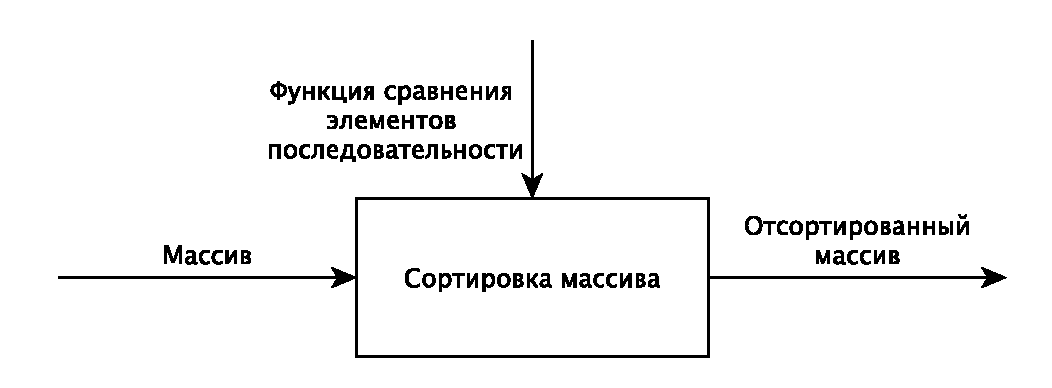
\includegraphics[scale=1]{./pictures/idef0.pdf}
\caption{Функциональная модель алгоритмов сортировки}
\end{figure}

\section{Разработка алгоритмов}
В данном разделе рассматриваются необходимые алгоритмы с помощью блок-схем.
\subsection{Поразрядная сортировка}
На рисунке 2.2 представлен алгоритм поразрядной сортировки.
\begin{figure}
\centering
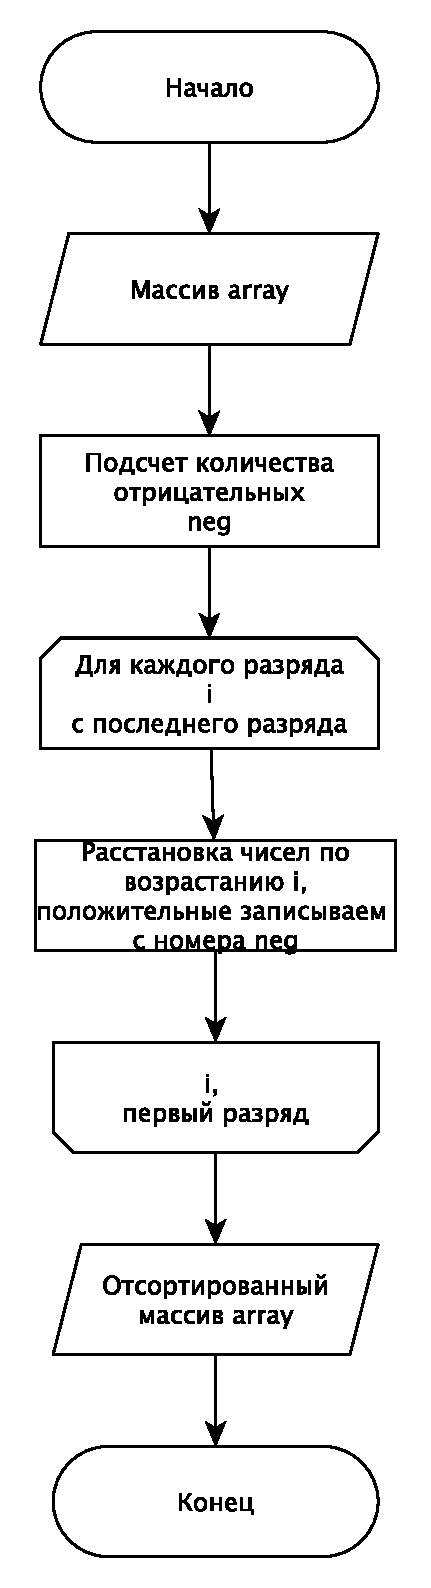
\includegraphics[scale=0.8]{./pictures/shema1.pdf}
\caption{Алгоритм поразрядной сортировки}
\end{figure}
\newpage
\subsection{Сортировка вставками}
На рисунке 2.3 представлен алгоритм сортировки вставками.
\begin{figure}[H]
\centering
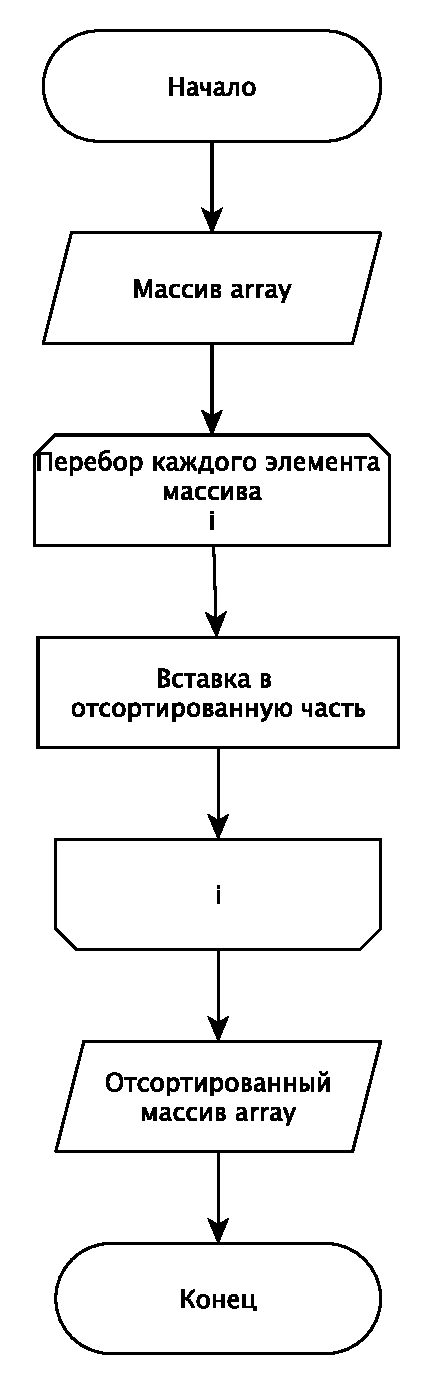
\includegraphics[scale=0.8]{./pictures/shema2.pdf}
\caption{Алгоритм сортировки вставками}
\end{figure}
\newpage
\subsection{Быстрая сортировка}
На рисунке 2.4 представлен алгоритм быстрой сортировки.
\begin{figure}[H]
\centering
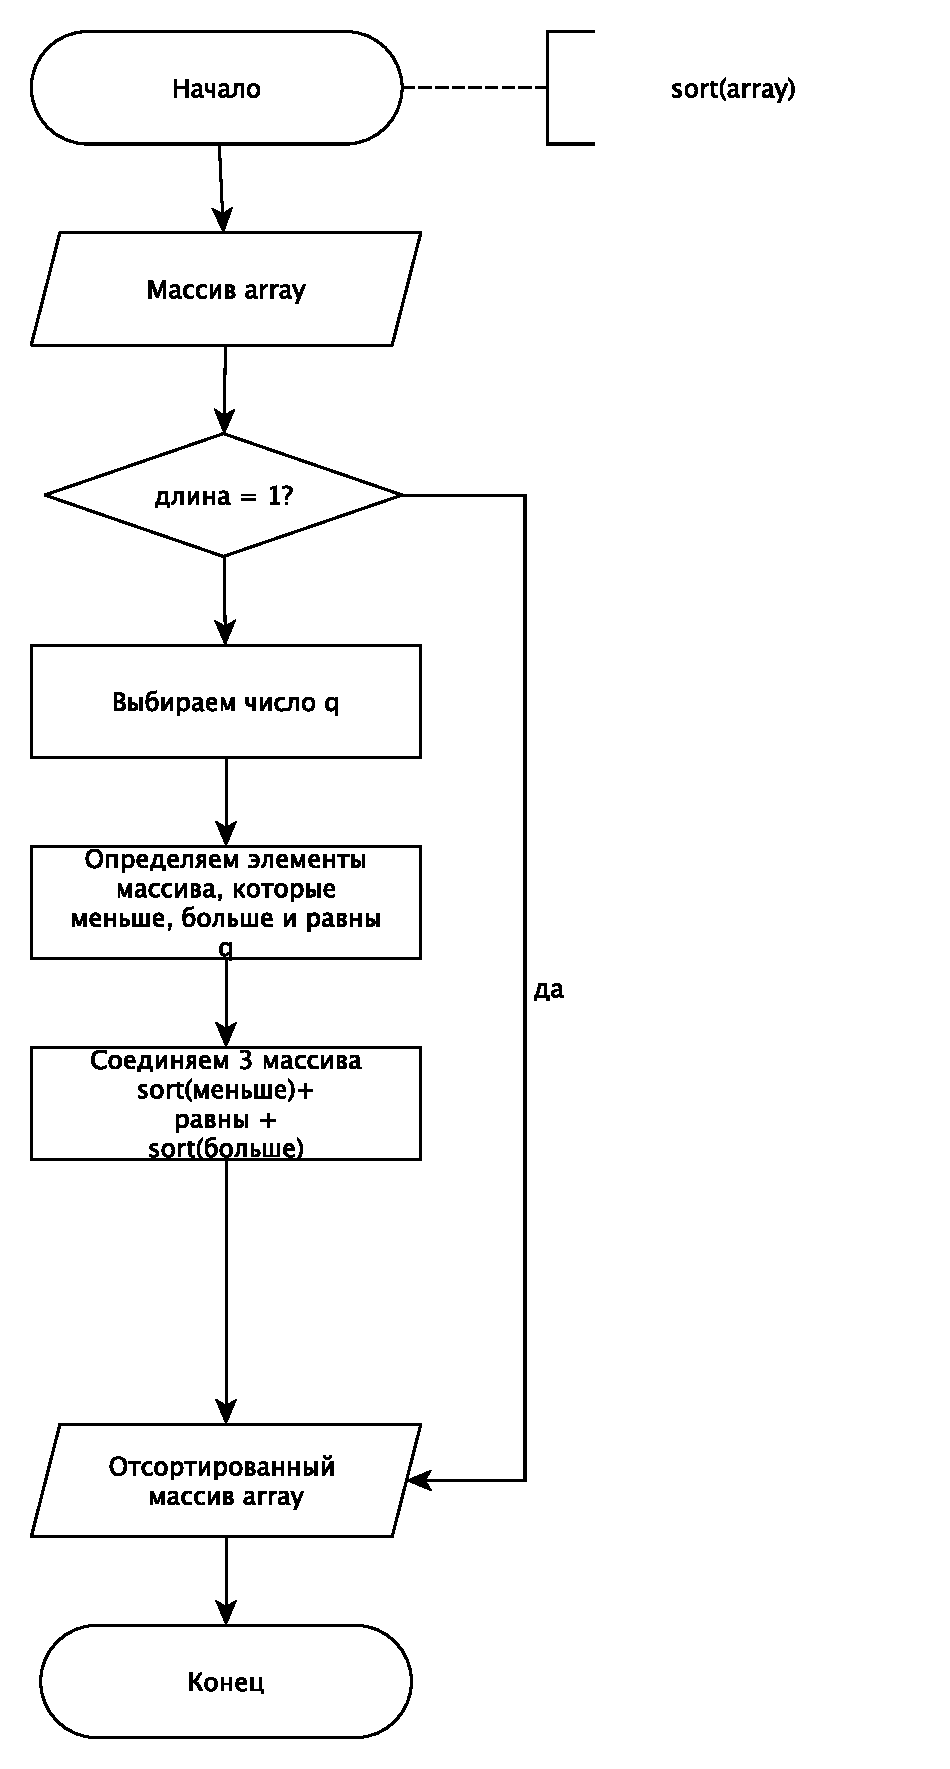
\includegraphics[scale=0.7]{./pictures/shema3.pdf}
\caption{Быстрая сортировка}
\end{figure}

\section{Сравнительный анализ алгоритмов}
	\begin{enumerate}
		\item Поразрядная сортировка 
		$$f=len + 2 + digit(2 +\underbrace{2 + len(2+1)}_{\text{расстановка}} + \underbrace{2 +digit(2+1)}_{\text{запись в массив}}=$$
		$$ = len+2 +digit(6+3len+2digit)=len+2+6digit+2digit^2+3digit\cdot len$$
		$$f = O(nk), n - \text{размер массива}, k- \text{порядок числа}$$
		$$\textbf{чем больше порядок числа тем больше трудоемкость}$$
		
		\item Сортировка вставками
		$$f=2+len(2+\underbrace{2+key(2+1)}_{\text{поиск позиции(сравнение)}}+\underbrace{1}_{\text{вставка}})=$$
		$$=2+len(5+3key)=2+5len+3len\cdot key$$
		$$f=O(n), n -\text{размер массива, }$$
        $$\text{Лучший случай - упорядоченный массив}$$
		$$f=O(n^2), n -\text{размер массива, }$$
        $$\text{Худший случай - обратноупорядоченный массив}$$
		$$f=O(n^2), n -\text{размер массива, }\text{Средний случай}$$
		
		\item Быстрая сортировка
		$$f=O(n \cdot ln(n)),, n -\text{размер массива, }$$
        $$\text{Лучший случай- упорядоченный массив}$$
		$$f=O(n^2), n -\text{размер массива, }$$
        $$\text{Худший случай - обратноупорядоченный массив}$$
		$$f=O(n \cdot ln(n)), n -\text{размер массива, }\text{Средний случай}$$
	\end{enumerate}
\subsection{Вывод}

	Вычислительная трудоемкость процедуры упорядочивания является достаточно высокой. Так, для ряда известных простых методов (пузырьковая сортировка, сортировка включением и др.) количество необходимых операций определяется квадратичной зависимостью от числа упорядочиваемых данных. Для более эффективных алгоритмов трудоемкость ниже. 
	
	Однако для различных сортировок можно получить меньшую трудоемкость на частных вариантах задачи.
